\documentclass[a4paper,12pt]{exam}
\usepackage{graphicx}
\usepackage{calc}
\usepackage{xcolor}
\usepackage[utf8x]{inputenc}
\usepackage{dirtree}
\usepackage[french]{babel}
\usepackage[T1]{fontenc}
\usepackage{amsfonts,amssymb}
\usepackage[margin=1cm,includeall]{geometry}
\parindent=0cm
\usepackage[french,ruled]{algorithm2e}
\usepackage{listings}
\usepackage{array,multirow,makecell}
\usepackage{colortbl}
\setcellgapes{1pt}
\usepackage{multicol}
\usepackage{wrapfig}
\usepackage{subcaption}
%\usepackage{fancyhdr}
\usepackage{appendix}
\makegapedcells
%\pagestyle{fancy}
%\renewcommand{\headrulewidth}{2pt}
%\renewcommand{\footrulewidth}{1pt}
\pagestyle{headandfoot}
\extraheadheight{1cm}
\headrule
\header{
\includegraphics[scale=1]{logo.png}}
				{}
				{Première, Spécialité Numérique et Sciences Informatiques}
\extrafootheight{1cm}
\footrule
\footer{
\includegraphics[scale=0.20]{cc.png}}
				{Séquence 4, Systèmes d'exploitation}
				{Page \thepage /\numpages}

\lstset{literate=
	{á}{{\'a}}1 {é}{{\'e}}1 {í}{{\'i}}1 {ó}{{\'o}}1 {ú}{{\'u}}1
	{Á}{{\'A}}1 {É}{{\'E}}1 {Í}{{\'I}}1 {Ó}{{\'O}}1 {Ú}{{\'U}}1
	{à}{{\`a}}1 {è}{{\`e}}1 {ì}{{\`i}}1 {ò}{{\`o}}1 {ù}{{\`u}}1
	{À}{{\`A}}1 {È}{{\'E}}1 {Ì}{{\`I}}1 {Ò}{{\`O}}1 {Ù}{{\`U}}1
	{ä}{{\"a}}1 {ë}{{\"e}}1 {ï}{{\"i}}1 {ö}{{\"o}}1 {ü}{{\"u}}1
	{Ä}{{\"A}}1 {Ë}{{\"E}}1 {Ï}{{\"I}}1 {Ö}{{\"O}}1 {Ü}{{\"U}}1
	{â}{{\^a}}1 {ê}{{\^e}}1 {î}{{\^i}}1 {ô}{{\^o}}1 {û}{{\^u}}1
	{Â}{{\^A}}1 {Ê}{{\^E}}1 {Î}{{\^I}}1 {Ô}{{\^O}}1 {Û}{{\^U}}1
	{Ã}{{\~A}}1 {ã}{{\~a}}1 {Õ}{{\~O}}1 {õ}{{\~o}}1
	{œ}{{\oe}}1 {Œ}{{\OE}}1 {æ}{{\ae}}1 {Æ}{{\AE}}1 {ß}{{\ss}}1
	{ű}{{\H{u}}}1 {Ű}{{\H{U}}}1 {ő}{{\H{o}}}1 {Ő}{{\H{O}}}1
	{ç}{{\c c}}1 {Ç}{{\c C}}1 {ø}{{\o}}1 {å}{{\r a}}1 {Å}{{\r A}}1
	{€}{{\euro}}1 {£}{{\pounds}}1 {«}{{\guillemotleft}}1
	{»}{{\guillemotright}}1 {ñ}{{\~n}}1 {Ñ}{{\~N}}1 {¿}{{?`}}1
	{~} {$\sim$}{1}
}
\title{Systèmes d'exploitation}
\author{Lycée Français de Tananarive}
\date{}

\begin{document}

%	\thispagestyle{fancy}
\maketitle
\thispagestyle{headandfoot}

\section{Principes Généraux}
\subsection{Définition}

\noindent\fcolorbox{black}{gray!30}{\parbox{\linewidth-2\fboxrule-2\fboxsep}
	{Un système d'exploitation est un programme ou un ensemble de programme dont le but est de gérer les ressources matérielles et logicielles d'un ordinateur. }}

\bigskip
\setlength{\parindent}{8ex}Le schéma ci-dessous (figure 1) indique la place du système d'exploitation et ses interactions. L'utilisateur interagit avec les applications, ces dernières ont besoin d'utiliser les ressources de la machine pour effectuer des tâches (lire ou sauvegarder des fichiers, afficher des images à l'écran, récupérer des caractères saisis au clavier ou la position du pointeur de la souris)
\begin{wrapfigure}{R}{0.3\textwidth}
	\centering
	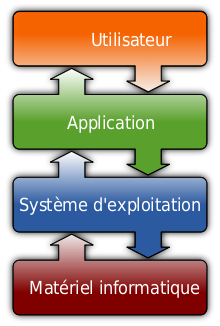
\includegraphics[width=0.2\textwidth]{os.png}
	\caption{}
\end{wrapfigure}
\subsection{Fonctionnalités d'un système d'exploitation}
Le système d'exploitation offre un ensemble de fonctions permettant d'interagir avec le matériel.
\bigskip

Parmi les différents composants d'un système d'exploitation on retrouve :
\begin{itemize}
	\item L'ordonnanceur qui décide quel programme s'exécute à un instant donné par le processeur.
	\item Le gestionnaire de mémoire, qui répartit la mémoire entre les différents programmes en cours d'exécution.
	\item les différents systèmes de fichiers, qui définissent la manière de stocker les fichiers sur les supports physiques.
	\item La pile réseau qui implémente entre autre des protocoles tel que TCP/IP
	\item les pilotes de périphériques (\textit{drivers}) qui gérent les périphériques matériel.
\end{itemize}
\vfill
\section{Questions sur les systèmes d'exploitation}
\begin{questions}
\question Donner le nom de chaque OS son logo (figure 2 ci-dessous)
		\newline
		1.\fillin[][10cm]
		\newline
		2.\fillin[][10cm]
		\newline
		3.\fillin[][10cm]
		\newline
		4.\fillin[][10cm]
		\newline
		5.\fillin[][10cm]
		
	\question Donnez la date approximative de création de chacun des OS suivant :
	\newline
	UNIX     \fillin[][10cm]
	\newline
	MS-DOS\fillin[][9.7cm]
	\newline
	Mac-OS \fillin[][9.8cm]
	\newline
	Linux \fillin[][10.2cm]
	\newline
	Windows \fillin[][9.6cm]
	\newline
	BSD \fillin[][10.4cm]
	\newline
	Android \fillin[][9.8cm]
	\question Que signifie POSIX ?
	\makeemptybox{3cm}
	\begin{figure}[h]
	\centering
	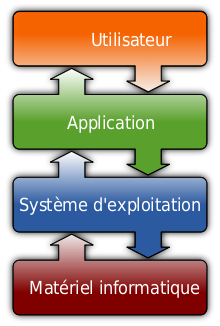
\includegraphics[width = 0.7\textwidth]{os.jpg}
	\caption{}
\end{figure}

\end{questions}
\end{document}
